
%(BEGIN_QUESTION)
% Copyright 2015, Tony R. Kuphaldt, released under the Creative Commons Attribution License (v 1.0)
% This means you may do almost anything with this work of mine, so long as you give me proper credit

Calculate the volume of liquid discharged from this vessel between 1:00 PM and 4:00 PM based on the information shown here:

$$\includegraphics[width=15.5cm]{i02889x01.eps}$$

$V_{discharged}$ between 1:00 PM and 4:00 PM = \underbar{\hskip 50pt} gallons

\vskip 10pt

\underbar{file i02889}
%(END_QUESTION)





%(BEGIN_ANSWER)

Here we are asked to calculate a total volume given flow rate (in gallons per minute) and time.  This involves multiplication (so that minutes of time will cancel out the "minutes" in GPM to yield an answer in gallons), which means the appropriate calculus function is {\it integration}.  Specifically, we need to integrate the flow rate of FT-240 over the time interval of 1:00 PM to 4:00 PM:  

$$V_{discharged} = \int_{1:00 \hbox{ PM}}^{4:00 \hbox{ PM}} Q_{FT-240} \> dt$$

This integral represents the area beneath the FT-240 flow function between 1:00 PM and 4:00 PM on the trend graph, represented by the two shaded rectangles below:

$$\includegraphics[width=15.5cm]{i02889x02.eps}$$

The first rectangle is 35 GPM high and 60 minutes wide, yielding an area of 2100 gallons:

$$\left(35 \hbox{ gal} \over \hbox{min} \right) \left(60 \hbox{ min} \over 1 \right) = 2100 \hbox{ gal}$$

\vskip 10pt

The second rectangle is 27.5 GPM high and 120 minutes wide, yielding an area of 3300 gallons:

$$\left(27.5 \hbox{ gal} \over \hbox{min} \right) \left(120 \hbox{ min} \over 1 \right) = 3300 \hbox{ gal}$$

\vskip 10pt

Together, the total area of these two rectangles is 5400 gallons, which is the value of our integral, and therefore the total quantity of liquid discharged from the vessel between 1:00 PM and 4:00 PM.

\vskip 10pt

$V_{discharged}$ between 1:00 PM and 4:00 PM = \underbar{\bf 5400} gallons

%(END_ANSWER)





%(BEGIN_NOTES)


%INDEX% Mathematics, calculus: integral (accumulated volume as the integral of flow)
%INDEX% Mathematics, calculus: integration (numerical)

%(END_NOTES)


